\documentclass[letterpaper,openany,oneside,twocolumn]{book}

\newcommand{\PATH}{../../}

\usepackage{fontspec}
\usepackage[justified]{\PATH dndtemplate/dnd}
\usepackage{ifthen}
\usepackage{pstricks}

\usepackage{intcalc}

\usepackage[UKenglish]{babel}
\usepackage{\PATH dndtemplate}

\setlength\oddsidemargin{\dimexpr(\paperwidth-\textwidth)/2 - 1in\relax}
\setlength\evensidemargin{\oddsidemargin}

% Headline
\CharacterName{Mehen (Leaper) Norixius}

\Class{Paladin}
\Level{3}
\Background{Outlander}
\PlayerName{M4RZ}
\Race{Gem Dragonborn}
\Alignment{Lawful Good}
\XP{}

% Ability scores (correct scores, no modifiers are automatically applied)
% Modifiers, Saving Throws and Skills are calculated automatically
\StrengthScore{17}
\DexterityScore{9}
\ConstitutionScore{13}
\IntelligenceScore{12}
\WisdomScore{11}
\CharismaScore{15}

% Proficiencies (Proficient = 'P', Expertise = 'E', otherwise = '')
\StrengthProficiency{}
\DexterityProficiency{}
\ConstitutionProficiency{}
\IntelligenceProficiency{}
\WisdomProficiency{P}
\CharismaProficiency{P}

\AcrobaticsProficiency{}
\AnimalHandlingProficiency{}
\ArcanaProficiency{}
\AthleticsProficiency{P}
\DeceptionProficiency{}
\HistoryProficiency{}
\InsightProficiency{}
\IntimidationProficiency{P}
\InvestigationProficiency{}
\MedicineProficiency{}
\NatureProficiency{}
\PerceptionProficiency{}
\PerformanceProficiency{}
\PersuasionProficiency{P}
\ReligionProficiency{}
\SleightOfHandProficiency{}
\StealthProficiency{}
\SurvivalProficiency{P}


\Inspiration{}
\Proficiency{+2}

% Armor Class is not automatically calculated
\ArmorClass{16}
\InitiativeModifier{0}
\Speed{30 ft}
\MaxHitPointsRolled{22} % Without Constitution Bonus, is added automatically
\CurrentHitPoints{}
\TemporaryHitPoints{}
\HitDice{d10}
\HitDiceSpent{0}

\CP{}
\SP{}
\EP{}
\GP{10}
\PP{}

% Weapon Arsenal
\AddWeapon{Greatsword}{0}{2d6 s}
\AddWeapon{\footnotesize{Spear of the Green}}{0}{1d6/1d8 p}

\def\BreathWeaponDamage{\ifthenelse{\LevelValue < 5}%
	{1d10}%
	{%
		\ifthenelse{\LevelValue < 11}%
		{2d10}%
		{%
			\ifthenelse{\LevelValue < 17}{3d10}{4d10}%
		}%	
	}%
}

\AttacksAdditional{
	\textbf{Greatsword}\\
	\textbf{Spear of the Green} (\textit{Throw, 1/2-Handed})\\
	\textbf{Armor:}\\
	Chain Mail (Stealth Disadvantage, STR 13), \textbf{Sentinel Shield} \\
	\\
	\textbf{Divine Sense} (\intcalcAdd{1}{\calculateModifier{\CharismaScoreValue}} uses) \\
	\textbf{Lay on Hands} (Health Pool: \intcalcMul{\LevelValue}{5}) \\
	\textbf{Divine Smite} \\
	\textbf{Breath Weapon} (Damage: \BreathWeaponDamage)
}

\OtherProficienciesLanguages{
\textbf{Languages:}\\Common, Draconic, Elvish\\
\textbf{Armor:}\\All Armor, Shields\\
\textbf{Weapons:}\\Simple Weapons, Martial Weapons\\
\textbf{Tools:}\\Long Horn
}

\Equipment{
	A staff,
	a hunting trap,
	a bear claw,
	a set of traveler's clothes,
	backpack,
	a bedroll,
	a mess kit,
	tinderbox,
	10 torches,
	10 days of rations,
	a waterskin,
	50 ft of hempen rope\\
	\textbf{Amulet with a Scale of Sardior}
}

\PersonalityTraits{
	I have a lesson for every situation, drawn from observing nature.
}

\Ideals{
	\textbf{Honor.} If I dishonor myself, I dishonor my whole clan. (Lawful)
}

\Bonds{
	I suffer awful visions of a coming disaster and will do anything to prevent it.
}

\Flaws{
	Don't expect me to save those who can't save themselves. It is nature's way that the strong thrive and the weak perish.
}

\FeaturesTraits{
\textbf{Gem Dragonborn Traits}
\begin{itemize}
	\item Breath Weapon
	\item Damage Resistance
	\item Psionic Mind
	\item Gem Flight
\end{itemize}
\textbf{Fighting Style}
\begin{itemize}
	\item Great Weapon Fighting
\end{itemize}
\textbf{Sacred Oath (Oath of the Ancients)}
\begin{itemize}
	\item Tenets of the Ancients
	\item Oath Spells
	\item Channel Divinity
	\begin{itemize}
		\item Nature's Wrath
		\item Turn the Faithless
	\end{itemize}
\end{itemize}
\textbf{Feats}
\begin{itemize}
	\item Gift of the Chromatic Dragon
\end{itemize}
}

% Appearance

\Age{37}
\Height{6'5''}
\Weight{240lbs}
\Eyes{Silver}
\Skin{Turquoise-Blue}
\Hair{}

% background

\CharacterAppearance{
	\begin{center}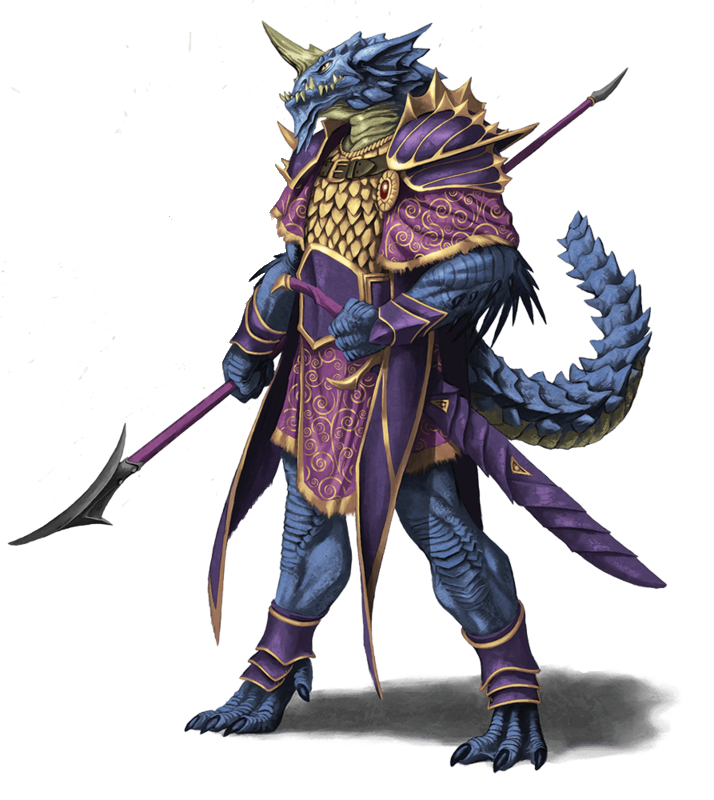
\includegraphics[width=125pt]{images/Mehen_Norixius.png}\end{center}
	\noindent Mehen Norixius is a 6'5'' tall Sapphire Gem Dragonborn. Covered in turquoise-blue scales he radiates a sturdy but noble appearance. Nothing escapes his silvery eyes and he is always aware of his surroundings.
}
\AdditionalFeaturesAndTraits{
	Lorem ipsum dolor sit amet, consectetur adipiscing elit, sed do eiusmod tempor incididunt ut labore et dolore magna aliqua. Nullam eget felis eget nunc lobortis mattis aliquam faucibus. Dictumst quisque sagittis purus sit. Mattis nunc sed blandit libero volutpat sed cras ornare. Blandit cursus risus at ultrices mi tempus imperdiet. Et netus et malesuada fames ac turpis egestas maecenas. Nibh cras pulvinar mattis nunc sed blandit. Varius vel pharetra vel turpis nunc eget lorem dolor. Tellus orci ac auctor augue. Nulla aliquet enim tortor at auctor urna nunc id cursus. A condimentum vitae sapien pellentesque habitant morbi tristique. Viverra suspendisse potenti nullam ac tortor. Quam lacus suspendisse faucibus interdum posuere lorem ipsum dolor. Nisl condimentum id venenatis a. Dui nunc mattis enim ut tellus elementum sagittis.
}
\Characterbackground{
	Lorem ipsum dolor sit amet, consectetur adipiscing elit, sed do eiusmod tempor incididunt ut labore et dolore magna aliqua. Nullam eget felis eget nunc lobortis mattis aliquam faucibus. Dictumst quisque sagittis purus sit. Mattis nunc sed blandit libero volutpat sed cras ornare. Blandit cursus risus at ultrices mi tempus imperdiet. Et netus et malesuada fames ac turpis egestas maecenas. Nibh cras pulvinar mattis nunc sed blandit. Varius vel pharetra vel turpis nunc eget lorem dolor. Tellus orci ac auctor augue. Nulla aliquet enim tortor at auctor urna nunc id cursus. A condimentum vitae sapien pellentesque habitant morbi tristique. Viverra suspendisse potenti nullam ac tortor. Quam lacus suspendisse faucibus interdum posuere lorem ipsum dolor. Nisl condimentum id venenatis a. Dui nunc mattis enim ut tellus elementum sagittis.
}
\Treasure{
	Lorem ipsum dolor sit amet, consectetur adipiscing elit, sed do eiusmod tempor incididunt ut labore et dolore magna aliqua. Nullam eget felis eget nunc lobortis mattis aliquam faucibus. Dictumst quisque sagittis purus sit. Mattis nunc sed blandit libero volutpat sed cras ornare. Blandit cursus risus at ultrices mi tempus imperdiet. Et netus et malesuada fames ac turpis egestas maecenas. Nibh cras pulvinar mattis nunc sed blandit. Varius vel pharetra vel turpis nunc eget lorem dolor. Tellus orci ac auctor augue. Nulla aliquet enim tortor at auctor urna nunc id cursus. A condimentum vitae sapien pellentesque habitant morbi tristique. Viverra suspendisse potenti nullam ac tortor. Quam lacus suspendisse faucibus interdum posuere lorem ipsum dolor. Nisl condimentum id venenatis a. Dui nunc mattis enim ut tellus elementum sagittis.
}
\AlliesAndOrganizations{
	The Oath of the Ancients is as old as the race of elves and the rituals of the druids. Sometimes called fey knights, green knights, or horned knights, paladins who swear this oath cast their lot with the side of the light in the cosmic struggle against darkness because they love the beautiful and life-giving things of the world, not necessarily because they believe in principles of honor, courage, and justice. They adorn their armor and clothing with images of growing things - leaves, antlers, or flowers - to reflect their commitment to preserving life and light in the world.
}
\OrganizationName{Oath of the Ancients}
\OrganizationSymbol{images/Oath_of_the_Ancients.png}

% Magic

\SpellcastingClass{Paladin}
\SpellcastingAbility{CHA} % STR, DEX, CON, INT, WIS, CHA
\SpellSaveDCModifier{0} % any modifier that isn't contained in "8 + Ability Modifier + Proficiency Bonus"

\FirstLevelSpellSlotsTotal{3}
\FirstLevelSpellSlotA{Cure Wounds (V, S)}
\FirstLevelSpellSlotB{Thunderous Smite (V)}
\FirstLevelSpellSlotC{Wrathful Smite (V)}
\FirstLevelSpellSlotD{Ensnaring Strike (V)}
\FirstLevelSpellSlotE{Speak with Animals (V, S)}

\begin{document}

\newgeometry{left=0cm,right=0cm,top=0cm,bottom=0cm}
\onecolumn


% CHARACTER PAGE
\rendercharactersheet

% BACKSTORY PAGE
\renderbackgroundsheet

% SPELLCASTING PAGE
\renderspellsheet


\restoregeometry
\twocolumn

\chapter*{Features, Magic Items and Spells}

\section*{Paladin}
\subsection*{Divine Sense}
The presence of strong evil registers on your senses like a noxious odor, and powerful good rings like heavenly music in your ears. As an action, you can open your awareness to detect such forces. Until the end of your next turn, you know the location of any celestial, fiend, or undead within 60 feet of you that is not behind total cover. You know the type (celestial, fiend, or undead) of any being whose presence you sense, but not its identity (the vampire Count Strahd von Zarovich, for instance). Within the same radius, you also detect the presence of any place or object that has been consecrated or desecrated, as with the Hallow spell.\\
You can use this feature a number of times equal to 1 + your Charisma modifier. When you finish a long rest, you regain all expended uses. (\textbf{Usages: \intcalcAdd{1}{\calculateModifier{\CharismaScoreValue}}})
\subsection*{Lay on Hands}
Your blessed touch can heal wounds. You have a pool of healing power that replenishes when you take a long rest. With that pool, you can restore a total number of hit points equal to your paladin level x 5.\\
As an action, you can touch a creature and draw power from the pool to restore a number of hit points to that creature, up to the maximum amount remaining in your pool.\\
Alternatively, you can expend 5 hit points from your pool of healing to cure the target of one disease or neutralize one poison affecting it. You can cure multiple diseases and neutralize multiple poisons with a single use of Lay on Hands, expending hit points separately for each one.\\
This feature has no effect on undead and constructs. \\
\textbf{(Healing Pool: \intcalcMul{\LevelValue}{5})}
\subsection*{Fighting Style}
Starting at 2nd level, you adopt a particular style of fighting as your specialty. Choose one of the following options. You can't take a Fighting Style option more than once, even if you later get to choose again.
\subsubsection*{Great Weapon Fighting}
When you roll a 1 or 2 on a damage die for an attack you make with a melee weapon that you are wielding with two hands, you can reroll the die and must use the new roll. The weapon must have the two-handed or versatile property for you to gain this benefit.
\subsection*{Divine Smite}
Starting at 2nd level, when you hit a creature with a melee weapon attack, you can expend one spell slot to deal radiant damage to the target, in addition to the weapon's damage. The extra damage is 2d8 for a 1st-level spell slot, plus 1d8 for each spell level higher than 1st, to a maximum of 5d8. The damage increases by 1d8 if the target is an undead or a fiend, to a maximum of 6d8.
\subsection*{Divine Health}
By 3rd level, the divine magic flowing through you makes you immune to disease.
\subsection*{Sacred Oath (Oath of the Ancients)}
When you reach 3rd level, you swear the oath that binds you as a paladin forever. Up to this time you have been in a preparatory stage, committed to the path but not yet sworn to it. Your choice grants you features at 3rd level and again at 7th, 15th, and 20th level. Those features include oath spells and the Channel Divinity feature.
\subsubsection*{Tenets of the Ancients}
The tenets of the Oath of the Ancients have been preserved for uncounted centuries. This oath emphasizes the principles of good above any concerns of law or chaos. Its four central principles are simple.
\subparagraph*{Kindle the Light}
Through your acts of mercy, kindness, and forgiveness, kindle the light of hope in the world, beating back despair.
\subparagraph*{Shelter the Light}
Where there is good, beauty, love, and laughter in the world, stand against the wickedness that would swallow it. Where life flourishes, stand against the forces that would render it barren.
\subparagraph*{Preserve Your Own Light}
Delight in song and laughter, in beauty and art. If you allow the light to die in your own heart, you can't preserve it in the world.
\subparagraph*{Be the Light}
Be a glorious beacon for all who live in despair. Let the light of your joy and courage shine forth in all your deeds.
\subsubsection*{Oath Spells}
You gain oath spells at the paladin levels listed.
\begin{DndTable}[header=Oath of the Ancients Spells]{lX}
\textbf{Paladin Level}  &\textbf{Spells}		\\
3rd						&Ensnaring Strike, Speak with Animals	\\
5th						&Moonbeam, Misty Step					\\
9th						&Plant Growth, Protection from Energy	\\
13th					&Ice Storm, Stoneskin					\\
17th					&Commune with Nature, Tree Stride		\\
\end{DndTable}
\subsubsection*{Channel Divinity}
When you take this oath at 3rd level, you gain the following two Channel Divinity options.
\subparagraph*{Nature's Wrath}
You can use your Channel Divinity to invoke primeval forces to ensnare a foe. As an action, you can cause spectral vines to spring up and reach for a creature within 10 feet of you that you can see. The creature must succeed on a Strength or Dexterity saving throw (its choice) or be restrained. While restrained by the vines, the creature repeats the saving throw at the end of each of its turns. On a success, it frees itself and the vines vanish.
\subparagraph*{Turn the Faithless}
You can use your Channel Divinity to utter ancient words that are painful for fey and fiends to hear. As an action, you present your holy symbol, and each fey or fiend within 30 feet of you that can hear you must make a Wisdom saving throw. On a failed save, the creature is turned for 1 minute or until it takes damage.

A turned creature must spend its turns trying to move as far away from you as it can, and it can't willingly move to a space within 30 feet of you. It also can't take reactions. For its action, it can use only the Dash action or try to escape from an effect that prevents it from moving. If there's nowhere to move, the creature can use the Dodge action.

If the creature's true form is concealed by an illusion, shapeshifting, or other effect, that form is revealed while it is turned.

\section*{Gem Dragonborn Traits}
Gem dragonborn partake of the heritage of gem dragons, who claim to be heirs of Sardior, the Ruby Dragon. The colors and mysterious powers of gem dragons — amethyst, crystal, emerald, sapphire, and topaz — gleam in these dragonborn's scaled skin and course through their veins. Theirs are the wonders of the mind, the force of will, the brilliant light of insight, and the resounding echo of discovery — but also the desiccation of despair.
\subsection*{Gem Ancestry}
\textbf{Sapphire} \\
You trace your ancestry to a Gem dragon, granting you a special magical affinity. Choose one type of dragon from the Gem Ancestry table. This determines the damage type for your other traits as shown in the table.
\subsection*{Breath Weapon (Fizban's Treasury of Dragons)}
\textbf{Thunder - 15 ft. cone (DEX Saving Throw, DC >= \intcalcAdd{8}{\intcalcAdd{\calculateModifier{\ConstitutionScoreValue}}{\ProficiencyValue}}, Damage: \BreathWeaponDamage )} \\
When you take the Attack action on your turn, you can replace one of your attacks with an exhalation of magical energy in a 15-foot cone. Each creature in that area must make a Dexterity saving throw (DC = 8 + your Constitution modifier + your proficiency bonus). On a failed save, the creature takes 1d10 damage of the type associated with your Gem Ancestry. On a successful save, it takes half as much damage. This damage increases by 1d10 when you reach 5th level (2d10), 11th level (3d10), and 17th level (4d10).
\subsection*{Damage Resistance}
You have Resistance to the \textbf{Thunder} damage type associated with your Draconic ancestry.
\subsection*{Psionic Mind}
You can telepathically speak to any creature you can see within 30 feet of you. You don't need to share a language with the creature, but the creature must be able to understand at least one language.
\subsection*{Gem Flight}
Starting at 5th level, you can use a bonus action to manifest spectral wings on your body. These wings last for 1 minute. For the duration, you gain a flying speed equal to your walking speed and can hover. Once you use this trait, you can't do so again until you finish a long rest.

\section*{Background}
\subsection*{Outlander}
You grew up in the wilds, far from civilization and the comforts of town and technology. You've witnessed the migration of herds larger than forests, survived weather more extreme than any city-dweller could comprehend, and enjoyed the solitude of being the only thinking creature for miles in any direction. The wilds are in your blood, whether you were a nomad, an explorer, a recluse, a hunter-gatherer, or even a marauder. Even in places where you don't know the specific features of the terrain, you know the ways of the wild.
\subparagraph*{Skill Proficiencies}
Athletics, Survival
\subparagraph*{Tool Proficiencies}
Long Horn
\subparagraph*{Equipment}
A staff, a hunting trap, a trophy from an animal you killed, a set of traveler's clothes, and a pouch containing 10gp
\subsubsection*{Feature: Wanderer}
You have an excellent memory for maps and geography, and you can always recall the general layout of terrain, settlements, and other features around you. In addition, you can find food and fresh water for yourself and up to five other people each day, provided that the land offers berries, small game, water, and so forth.

\section*{Feats}
\subsection*{Gift of the Chromatic Dragon}
You've manifested some of the power of chromatic dragons, granting you the following benefits:
\subparagraph*{Chromatic Infusion}
As a bonus action, you can touch a simple or martial weapon and infuse it with one of the following damage types: acid, cold, fire, lightning, or poison. For the next minute, the weapon deals an extra 1d4 damage of the chosen type when it hits. After you use this bonus action, you can't do so again until you finish a long rest.
\subparagraph*{Reactive Resistance}
When you take acid, cold, fire, lightning, or poison damage, you can use your reaction to give yourself resistance to that instance of damage. You can use this reaction a number of times equal to your proficiency bonus, and you regain all expended uses when you finish a long rest.

\section*{Magical Items}
\subsection*{Spear of the Green}
Weapon \textit{(spear)}, \textit{legendary (requires attunement by a paladin)}\\
You gain a +3 bonus to attack and damage rolls made with this magic weapon. When you cast a paladin spell with a target of Self, you can't lose concentration on the spell from taking damage.\\
While you hold the drawn spear, it creates an aura in a 10-foot radius around you. Creatures of your choice in that aura gain resistance to poison damage and have advantage on saving throws against the poisoned condition. If you have 17 or more levels in the paladin class, the radius of the aura increases to 30 feet.
\subsection*{Sentinel Shield}
Armor \textit{(shield)}, \textit{uncommon}\\
While holding this shield, you have advantage on initiative rolls and Wisdom (Perception) checks. The shield is emblazoned with the symbol of an eye.
\subsection*{Amulet with a Scale of Sardior}
Is the holy symbol of this character and can be used as a \textit{Spellcasting Focus}. A Spellcasting Focus eliminates the need of most components of a spell, except major components with a GP value.

\section*{Spells}
\subsection*{Level 1}

\DndSpellHeader
  {Cure Wounds}
  {1st-Level Evocation}
  {1 Action}
  {Touch}
  {V, S}
  {Instantaneous}

A creature you touch regains a number of hit points equal to 1d8 + your spellcasting ability modifier. This spell has no effect on undead or constructs.

\subparagraph*{At Higher Levels} When you cast this spell using a spell slot of 2nd level or higher, the Healing increases by 1d8 for each slot level above 1st.

\DndSpellHeader
  {Thunderous Smite}
  {1st-Level Evocation}
  {1 Bonus Action}
  {Self}
  {V}
  {Concentration, up to 1 minute}

The first time you hit with a melee weapon attack during this spell's duration, your weapon rings with thunder that is audible within 300 feet of you, and the attack deals an extra 2d6 thunder damage to the target. Additionally, if the target is a creature, it must succeed on a Strength saving throw or be pushed 10 feet away from you and knocked prone.

\DndSpellHeader
  {Wrathful Smite}
  {1st-Level Evocation}
  {1 Bonus Action}
  {Self}
  {V}
  {Concentration, up to 1 minute}

The next time you hit with a melee weapon attack during this spell's duration, your attack deals an extra 1d6 psychic damage. Additionally, if the target is a creature, it must make a Wisdom saving throw or be frightened of you until the spell ends. As an action, the creature can make a Wisdom check against your spell save DC to steel its resolve and end this spell.

\DndSpellHeader
  {Ensnaring Strike}
  {1st-Level Conjuration}
  {1 Bonus Action}
  {Self}
  {V}
  {Concentration, up to 1 minute}

The next time you hit a creature with a weapon attack before this spell ends, a writhing mass of thorny vines appears at the point of impact, and the target must succeed on a Strength saving throw or be restrained by the magical vines until the spell ends. A Large or larger creature has advantage on this saving throw. If the target succeeds on the save, the vines shrivel away.

While restrained by this spell, the target takes 1d6 piercing damage at the start of each of its turns. A creature restrained by the vines or one that can touch the creature can use its action to make a Strength check against your spell save DC. On a success, the target is freed.

\subparagraph*{At Higher Levels} If you cast this spell using a spell slot of 2nd level or higher, the damage increases by 1d6 for each slot level above 1st.

\DndSpellHeader
  {Speak with Animals}
  {1st-Level Divination (Ritual)}
  {1 Action}
  {Self}
  {V, S}
  {10 minute}

You gain the ability to comprehend and verbally communicate with beasts for the duration. The knowledge and awareness of many beasts is limited by their intelligence, but at minimum, beasts can give you information about nearby locations and monsters, including whatever they can perceive or have perceived within the past day. You might be able to persuade a beast to perform a small favor for you, at the GM's discretion.

\section*{Miscellaneous}
\subsection*{Attack and Damage Rolls}
\subsubsection*{Battleaxe}
\paragraph*{Attack Roll} \hfill\\
1d20 + STR-Modifier + Proficiency Modifier
Current Max: \intcalcAdd{20}{\intcalcAdd{\calculateModifier{\StrengthScoreValue}}{\ProficiencyValue}}
\paragraph*{Damage Roll} \hfill\\
2d6 + STR-Modifier \\
Current Max: \intcalcAdd{\intcalcMul{2}{6}}{\calculateModifier{\StrengthScoreValue}}
\subsubsection*{Spear}
\paragraph*{Attack Roll} \hfill\\
1d20 + STR-Modifier + Proficiency Modifier \\
Current Max: \intcalcAdd{20}{\intcalcAdd{\calculateModifier{\StrengthScoreValue}}{\ProficiencyValue}}
\paragraph*{Damage Roll} \hfill\\
\textit{One-Handed or Thrown} \\
1d6 + STR-Modifier \\
Current Max: \intcalcAdd{6}{\calculateModifier{\StrengthScoreValue}}\\
\textit{Two-Handed} \\
1d8 + STR-Modifier \\
Current Max: \intcalcAdd{8}{\calculateModifier{\StrengthScoreValue}}

\end{document}
